% main.tex -- LNCS-format paper skeleton for the Ultrasound Biometry
% Foundation Model work (DINOv2 SSL domain adaptation + HRNet-style neck).
% Based on Springer's llncs.cls / samplepaper.tex (v2.21, 2022/01/12).
%
% Compile with pdflatex + bibtex, e.g.:
%   pdflatex main && bibtex main && pdflatex main && pdflatex main
%
\documentclass[runningheads]{llncs}

\usepackage[T1]{fontenc}
\usepackage{microtype} % better justification/hyphenation -- fixes several
                       % overfull-hbox margin overflows (e.g. long compound
                       % hyphenated words like "task-homogeneous") without
                       % changing any wording
\usepackage{graphicx}
\usepackage{amsmath}
\usepackage{cite} % auto-sorts + range-compresses multi-citations, e.g. [4-6,9]
\usepackage{booktabs}   % clean horizontal-rule tables (\toprule/\midrule/\bottomrule)
\usepackage{multirow}   % multi-row cells (clinical-domain grouping in tab:codabench-results)
\usepackage{subcaption} % side-by-side subfigures, if needed later
\raggedbottom           % disable flushbottom's inter-paragraph stretch glue --
                        % without this, sparsely-filled pages (e.g. the
                        % Introduction) visibly space paragraphs further apart
                        % than dense pages, even though the source formatting
                        % is identical
%\usepackage{float}      % [H] float placement -- keeps tables/figures exactly
                        % where declared in the source instead of drifting to
                        % the top of a later page (matters while sections are
                        % still placeholder-only with little body text)

% Uncomment for blue, roman-font hyperlinks per Springer's eBook style:
%\usepackage{color}
%\usepackage{hyperref}
%\renewcommand\UrlFont{\color{blue}\rmfamily}
%\urlstyle{rm}

\begin{document}

\title{Self-Supervised Domain Adaptation with DINOv2-HRNet for Multi-Task Ultrasound Landmark Detection}
\titlerunning{SSL Domain Adaptation with DINOv2-HRNet for Ultrasound Landmarks}

\author{Anna Panagiotakopoulou\inst{1}\orcidID{0009-0006-0957-6331}\thanks{Code available at: \texttt{https://github.com/abarmper/US-Foundation}} \and
Alexandros Barmperis\inst{1,2}\orcidID{0009-0000-6319-0700} \and
Vasileios E. Katsigiannis\inst{1}\orcidID{0009-0003-7464-0959} \and
George K. Matsopoulos\inst{1}\orcidID{0000-0002-2600-9914}}

\authorrunning{A. Panagiotakopoulou et al.}

%\institute{Your Institution, City, Country\\
\institute{Biomedical Engineering Laboratory, School of Electrical and Computer Engineering, \\
National Technical University of Athens, Athens, Greece\\
%\email{you@institution.edu}}
\email{annapan@biomed.ntua.gr, amparmperis@biomed.ntua.gr,
vassiliskat@biomed.ntua.gr, gmatsopoulos@biomed.ntua.gr} \and
Archimedes Research Unit, Athena Research Center, Athens, Greece}

\maketitle

\begin{abstract}
Accurate ultrasound biometry relies on precise anatomical landmark localization, yet building a unified model across heterogeneous ultrasound tasks remains challenging. Image appearance, acquisition protocols, and anatomical scale vary substantially across clinical domains, exacerbated by the severe scarcity of large-scale annotated datasets. To address the Generalization-oriented Ultrasound Biometry Challenge, we propose a two-stage foundation-model pipeline for generalizable multi-task landmark detection across nine diverse clinical tasks. Rather than treating each task as an isolated problem, we formulate biometry as cross-domain representation learning under limited keypoint supervision and distribution shift. First, a DINOv2 encoder is adapted on unlabeled ultrasound frames via DINO-style multi-crop self-distillation between a trainable student and an EMA teacher, capturing domain-specific sonographic textures without eroding the foundation model's semantic priors. Second, the adapted encoder is coupled with a domain-agnostic, HRNet-style multi-resolution neck designed to reconstruct localization-relevant spatial hierarchies directly from transformer patch features. Task-specific convolutional heads then utilize soft-argmax for direct, sub-pixel coordinate regression.

\keywords{Ultrasound biometry \and Self-supervised learning \and DINOv2 \and
Landmark localization \and HRNet.}
\end{abstract}


\section{Introduction}
Ultrasound biometry converts a small set of anatomical landmarks into clinically meaningful measurements, such as fetal biometric parameters~\cite{salomon2019isuog}, labor progression indices~\cite{ghi2018isuog}, and cardiac structural measurements~\cite{mitchell2019comprehensive}. Landmark localization has been studied extensively with single-task models~\cite{avisdris2022biometrynet,bai2026iugc,smistad2020real,yim2024assessment}, but multi-centre benchmarks reveal that site and scanner variability substantially degrades generalization~\cite{bai2026beyond,divece2026multicentre}. This heterogeneity renders task-specific supervision insufficient, motivating the need for a unified pipeline that can preserve spatial accuracy and measurement reliability under the cross-domain distribution shift central to the challenge (GU\_Biometry)~\cite{gu_biometry,deng2026baseline}.

Foundation models have advanced medical image analysis through reusable representation learning from unlabeled data: self-supervised transformers like DINOv2 learn transferable visual features without manual labels~\cite{oquab2023dinov2}, though direct transfer to sonography remains challenging given ultrasound's distinct texture statistics, acquisition physics, and artifacts~\cite{guan2022domain,wang2021deep}. Recent ultrasound foundation models~\cite{jiao2024usfm,ambsdorf2025general,maani2025fetalclip,jiang2025ultrafedfm} motivate domain-specific pretraining, but primarily target image-level classification, dense prediction, or few-shot analysis, leaving unified sparse landmark localization across biometric domains underexplored.

Landmark-based biometry requires global context alongside fine spatial precision. Vision Transformers extract robust features~\cite{dosovitskiy2021image,oquab2023dinov2} and have been adapted for keypoints (e.g., TransPose~\cite{yang2021transpose}, ViTPose~\cite{xu2022vitpose}). However, their coarse tokenization reduces native spatial resolution, making precise coordinate localization more challenging; even hierarchical variants such as Swin~\cite{liu2021swin} rely on progressive downsampling. We therefore pair foundation model features with a High-Resolution Network (HRNet)-style multi-resolution neck~\cite{sun2019hrnet}, preferred over standard U-Net architectures to maintain continuous high-resolution spatial detail throughout the network, critical for fine coordinate estimation.

Our main contributions are: (i) a two-stage DINOv2-HRNet pipeline that separates domain-level ultrasound representation learning from task-specific spatial localization; (ii) a study of how unlabeled self-supervised learning (SSL) adaptation duration affects downstream landmark accuracy; (iii) a metric-aligned validation strategy that selects checkpoints on the challenge's macro-averaged, per-task-normalized objective.

\section{Methodology}

\begin{figure}[tb]
\centering
\includegraphics[width=\textwidth]{Phase1_new-Page-1.pdf}
\caption{Phase 1 self-supervised pretraining: a trainable student and an EMA teacher process asymmetric multi-crop views through a shared encoder-pool-head pipeline. The teacher's raw logits are centered and sharpened into target probabilities under stop-gradient; the student's are temperature-scaled and log-softmaxed. The resulting cross-entropy loss backpropagates into the student only---the teacher updates solely via EMA of the student's parameters---and the student's encoder is periodically checkpointed.}
\label{fig:pipeline}
\end{figure}

\subsection{Phase 1: Self-Supervised Domain Adaptation}
\label{sec:phase1}

We adapt the register-variant DINOv2-L/14 encoder~\cite{oquab2023dinov2} to unlabeled ultrasound frames using DINO-style multi-crop self-distillation~\cite{caron2021dino}. To enforce scale invariance, we adopt a local-to-global distillation strategy that generates eight augmented views ($V$). Two \emph{global} crops cover 50--100\% of the image area and are resized to $518\times518$, while six \emph{local} crops cover 10--40\% of the area and are resized to $98\times98$. All views are produced using independent random resize crops, affine transformations, and photometric augmentations. During pre-training, only the student network processes the local crops, encouraging the student to infer global anatomical context from localized, texture-dominated patches---particularly relevant in sonography, where the model must correlate local speckle signatures with anatomical geometries.

A trainable student processes all 8 views, while an exponential-moving-average (EMA) teacher processes only the 2 global views. Both branches mean-pool their patch-token output and project it through a shared-architecture two-layer MLP head into a $256$-d embedding, $z_s^{(j)}$ for the student's view $j$ and $z_t^{(i)}$ for the teacher's view $i$. The teacher's target is centered against a running batch-mean estimate $c$ (EMA momentum $0.9$, preventing collapse) and sharpened at temperature $\tau_t{=}0.04$, giving target $q_i = \mathrm{softmax}\big((z_t^{(i)}-c)/\tau_t\big)$; the student predicts $p_j = \mathrm{softmax}\big(z_s^{(j)}/\tau_s\big)$ at temperature $\tau_s{=}0.1$. The student is optimized to match the teacher's distribution from every view except its own matching global crop---forcing consistency between the student's global-\emph{and}-local views and the teacher's global-only view:

\begin{equation}
\mathcal{L}_{\text{SSL}} = \sum_{i=1}^{2}\ \sum_{\substack{j=1 \\ j \neq i}}^{V} -\, q_i \log p_j.
\label{eq:ssl-loss}
\end{equation}
The teacher receives no gradient; it is instead updated as $\theta_t \leftarrow a\,\theta_t + (1-a)\,\theta_s$, with $a$ annealed from $0.99$ to $1.0$ on a cosine schedule over training (Figure~\ref{fig:pipeline}). Extended self-distillation exposure risks representational drift away from the foundation priors. 

\subsection{Phase 2: Multi-Stage HRNet Neck}
\label{sec:phase2}
To recover fine spatial resolution from the coarse $37\times37$ transformer tokens, we implement a multi-stage HRNet-style neck: parallel, multi-resolution branches that repeatedly exchange information bidirectionally, rather than being computed independently and fused only once (Figure~\ref{fig:neck-zoom}).

\begin{figure}[tb]
\centering
\includegraphics[width=\textwidth]{FIGURE2_UPDATED-Page-5.drawio.pdf}
%\caption{Detailed view of Phase 2 (expanding the "Neck" and "Regression" black boxes of Fig.~\ref{fig:pipeline}): branch spawning, the two exchange units, and the final multi-scale fusion into a $148\times148$, 128-channel representation, followed by task routing, the nine task-specific heads, and soft-argmax coordinate decoding.}
\caption{Detailed Phase~2 architecture: HRNet-style branch spawning and exchange, multi-scale fusion into a $148\times148$, 128-channel feature map, task routing, task-specific heads, and soft-argmax coordinate decoding.}
\label{fig:neck-zoom}
\end{figure}

Given a $518\times518$ input, the adapted register-variant DINOv2-L/14 encoder outputs, at every one of its 24 transformer blocks, a $37\times37$ grid of 1024-dimensional patch tokens (matching the encoder's 14-pixel patch stride); spatial resolution is constant with depth, only token semantics change. We tap four intermediate depths---blocks 5, 11, 17, and 23---and route each $37\times37\times1024$ grid directly into the neck's branch-spawning convolutions, which perform channel compression and spatial projection simultaneously without a dedicated $1\times1$ bottleneck.
Unlike standard HRNet designs, which build multi-resolution features bottom-up from image-space representations, our neck operates top-down from these already-semantic $37\times37$ DINOv2 token grids: higher-resolution branches are expanded outward from coarse features rather than obtained by progressive downsampling. Concretely, $B_1$ ($37\times37$) and $B_2$ ($74\times74$) are spawned directly and simultaneously from the two deepest taps---block 23 and block 17, respectively---via independent convolutional and transposed-convolutional projections, followed by an initial bidirectional exchange. $B_3$ ($148\times148$) is instead bootstrapped independently from the two shallowest taps (blocks 11 and 5), each projected through its own two-stage transposed-convolution stack and summed---rather than derived from $B_2$---after which all three branches participate in a dense all-pairs exchange.
Downsampling paths use chained stride-2 $3\times3$ convolutions with GroupNorm: a single stride-2 step for a $2\times$ resolution gap and two chained steps for a $4\times$ gap, avoiding a single stride-4 projection. Each upsampling path uses a $1\times1$ channel projection followed by bilinear interpolation. Each branch is updated by summing its own features with the resampled projections of the other branch(es), followed by ReLU: the two-branch exchange updates $b_1$ and $b_2$ this way, and the three-branch, all-pairs exchange applies the analogous update to each of $b_1$, $b_2$, and $b_3$. This bidirectional exchange serves a concrete purpose for ultrasound, since the coarse-to-fine path gives the high-resolution branches a semantic anchor so fine-detail detection is less likely to latch onto speckle noise or acoustic shadowing as if it were a real edge, while the fine-to-coarse path feeds sharp structural boundaries back to the coarse branch, preventing its semantic map from becoming under-localized.
Because training batches are task-homogeneous, BatchNorm's running statistics would become an average blended across all nine heterogeneous task distributions, poorly matching any single task's features at inference. We therefore use GroupNorm throughout the neck and task heads, since it normalizes per sample and does not depend on the other images in the batch.

\subsection{Task-Specific Heads and Coordinate Extraction}
After the final exchange, all branches are aligned to a common $148\times148$, 128-channel representation: $B_1$ and $B_2$ are projected and bilinearly upsampled, while $B_3$ is channel-projected only; the three are then fused by element-wise summation. Each task-homogeneous batch is then dispatched, by its (sampler-guaranteed) task identity rather than a learned routing mechanism, to one of nine independent task-specific heads. Each head applies two Conv-GroupNorm-ReLU blocks with 2D dropout to the fused $148\times148$ representation, and produces per-keypoint logits $\ell_k$ via a final $1\times1$ projection.

Coordinates are then extracted via soft-argmax, a temperature-scaled softmax over the flattened logits treated as a differentiable spatial expectation~\cite{nibali2018numerical}:
\begin{equation}
p_k = \text{softmax}(\tau \cdot \ell_k), \qquad
(\hat{x}_k, \hat{y}_k) = \Big(\sum_{(u,v)} p_k(u,v)\, u,\ \sum_{(u,v)} p_k(u,v)\, v\Big) \cdot \frac{518}{H},
\label{eq:softargmax}
\end{equation}
with temperature $\tau=10.0$ and $H$ the logit resolution ($148$). At inference these canvas-space coordinates are inverse-letterboxed back to original-image pixels---the space the official challenge metric is computed in---so validation, checkpoint selection, and reporting all optimize the real objective rather than a canvas-space proxy. The model is trained with a masked $L_1$ loss, reweighted per sample by that image's own letterbox scale factor ($\max(h,w)/\text{canvas}$) so residuals are measured in original-pixel units matching the metric's scale, over the visible keypoints $\mathcal{K}$ of the current task, plus a light differentiable spatial-to-numerical transform (DSNT)-style regularizer~\cite{nibali2018numerical} that keeps each predicted heatmap tight and unimodal without reintroducing a fixed heatmap-matching target. Unlike direct fully-connected regression, which discards spatial feature maps, or standard heatmap matching, which suffers from argmax quantization errors, soft-argmax yields continuous, sub-pixel coordinates directly from the probability map. This entirely avoids the need for empirical tuning of target-heatmap Gaussian scales.

%%%%%%%%%%%%%%%%%%%%%%%%%%%%%%%%%%%%%%

\section{Experiments}
\subsection{Dataset and Preprocessing}
We evaluate on the GU\_Biometry MICCAI 2026 Challenge dataset~\cite{gu_biometry}, spanning multi-vendor 2D ultrasound across three clinical domains (intrapartum, prenatal, and cardiac) and nine distinct biometric tasks, each defining landmarks for a different clinical measurement. The released training data comprise 197{,}938 images in total: 6{,}768 labeled and 191{,}170 unlabeled (a $\sim$3.4\% labeled fraction). Both pools are highly imbalanced across tasks: labeled counts range from $\sim$4{,}000 (AoP) to under 100 (IVC, PLAX, PSAX), and unlabeled counts are similarly skewed---fetal femur has none at all. For supervised training, the labeled set is split 80\%/20\%, yielding 5{,}414 training and 1{,}354 validation images.

Native image sizes vary substantially across tasks (e.g., median $336\times544$ for FUGC to $768\times1024$ for FA); to preserve landmark geometry for the DINOv2 encoder, all images undergo an aspect-ratio-preserving resize and zero-padding to a $518\times518$ canvas, followed by ImageNet pixel normalization. On top of this base preprocessing, Phase~2 supervised training applies moderate augmentation (affine scale up to $\pm5\%$, translation up to $\pm10\%$, rotation up to $\pm30^\circ$, brightness/contrast $\pm0.2$, a gamma-or-CLAHE choice, and light Gaussian noise), Phase~1 unlabeled adaptation applies a stronger, fixed recipe (rotation up to $\pm45^\circ$, gamma/contrast changes, CLAHE, Gaussian blur and noise) to encourage robustness to acquisition variability, and validation and inference use only the base preprocessing, with no augmentation.

\subsection{Implementation Details}
All experiments were executed on a single NVIDIA A100-SXM4-80GB GPU with a batch size of 64. Training uses bf16 mixed precision with gradient-norm clipping and AdamW (weight decay excluded on norm/bias parameters, dimensionality $<2$; base LR $2\times10^{-4}$, 15-epoch linear warmup, 150-epoch cosine decay). The backbone uses layer-wise learning rate decay (LLRD, factor $0.75$), starting at $0.1\times$ base LR for the last four unfrozen blocks. A Phase~2 EMA teacher ($\alpha=0.999$) is maintained for stabilized validation, early stopping (patience 40), and final inference. A temperature-scaled ($\tau=0.5$) task-homogeneous sampler allocates per-task batches in proportion to (task size)$^{0.5}$, damping AoP's $\sim$40$\times$ raw imbalance over the smallest cardiac tasks to a $\sim$6$\times$ replay-rate gap. Checkpoint selection directly optimizes a macro-averaged, per-task-normalized blend of landmark and clinical-measurement error in original-pixel space, mirroring the official challenge scoring; final reported results use the same native-resolution metric, evaluated by the official Codabench server.

%%%%%%%%%%%%%%%%%%%%%%%%%%%%%%%%%%%%%%%%%%%

\section{Results}

% ============================================================
% Results narrative: two cheap fold-0 searches, then one final
% validated 5-fold+TTA run. Steps 1-2 use the LOCAL scorer
% (metrics.py, verified to reproduce official local_eval) on
% fold 0's held-out split -- no Codabench submissions spent on
% search. Step 3 is the official Codabench submission.
% ============================================================

\subsection{Phase-1 Checkpoint Duration Selection}
\label{sec:ssl-duration}
To select the Phase-1 adaptation duration used for all subsequent experiments, we compare the epoch-10 and epoch-20 checkpoints as Phase-2 initializations, training the baseline Phase-2 recipe on fold~0 and scoring on that fold's held-out validation split with our local challenge-metric scorer (Section~\ref{sec:phase2}). Table~\ref{tab:phase1-phase2} reports the results: the epoch-20 checkpoint performs better across all metrics and is the Phase-1 initialization used for the final model. Qualitative PCA of patch-token feature maps are shown in Figure~\ref{fig:feature-maps}.

\begin{table}[tb]
\caption{Fold-0 internal validation: Phase-1 checkpoint duration (left, baseline recipe) and Phase-2 recipe (right, epoch-10 checkpoint), side by side. Mean radial error (MRE, px) and mean absolute clinical-measurement error (AvgMAE), macro-averaged over all nine tasks.}
\label{tab:phase1-phase2}
\centering
\begin{tabular}{@{}lcc|lcc@{}}
\toprule
Phase-1 checkpoint & epoch 10 & epoch 20 & Phase-2 recipe & Baseline & Upgraded \\
\midrule
Mean MRE & 40.32 & \textbf{33.95} & Mean MRE & 40.32 & \textbf{31.12} \\
Mean AvgMAE & 25.33 & \textbf{23.37} & Mean AvgMAE & 25.33 & \textbf{22.52} \\
\bottomrule
\end{tabular}
\end{table}

\begin{figure}[tb]
\centering
\includegraphics[width=\textwidth]{fig3_variant_seed1.pdf}
\caption{Original ultrasound frames and their corresponding DINOv2 patch-token PCA feature maps at the epoch-10 and epoch-20.}
\label{fig:feature-maps}
\end{figure}

\subsection{Phase-2 Recipe Selection}
\label{sec:phase2-recipe}
The Phase-1 initialization is fixed at the epoch-10 checkpoint. To isolate the Phase-2-specific upgrades from the backbone choice, both configurations use the register-variant backbone. We then compare the baseline Phase-2 recipe (single-mode neck, $128\times128$ heatmap, without LLRD, canvas-space loss, without DSNT) against the upgraded recipe (multilevel neck, $148\times148$ heatmap, LLRD $0.75$, original-pixel loss, DSNT $0.1$), on fold~0 only with the same local scorer. Table~\ref{tab:phase1-phase2} reports the results, where the upgraded recipe improves both MRE and AvgMAE and is carried forward to the final model.

\subsection{Official Challenge Evaluation}
Using the best Phase-1 checkpoint (Table~\ref{tab:phase1-phase2}) and the upgraded Phase-2 recipe, we submit a single model to the official Codabench evaluation (Table~\ref{tab:codabench-results}).

Table~\ref{tab:codabench-results} shows that performance varies substantially across domains, reflecting the heterogeneity of anatomy, data scarcity, and task-specific annotation structure.
Figure~\ref{fig:best-per-task} shows examples for four tasks spanning different clinical domains, illustrating the high-performing localization behavior of the final model.

\begin{table}[tb]
\caption{Official GU\_Biometry Codabench evaluation per task.}
\label{tab:codabench-results}
\centering
\begin{tabular}{llrrr}
\toprule
\textbf{Clinical domain} & \textbf{Task / Target view} & \textbf{$N$} & \textbf{MRE $\downarrow$} & \textbf{MAE $\downarrow$} \\
\midrule
\multicolumn{5}{l}{\textbf{Prenatal \& Gynecologic}} \\
 & Head Circumference (HC) & 215 & 45.20 & 59.64 \\
 & Fetal Abdomen (FA)      & 188 & 28.38 & 89.30 \\
 & Fetal Femur             & 62  & 27.38 & 18.24 \\
 & Cervical Segm. (FUGC)   & 20  & 13.79 & 10.63 \\
\midrule
\multicolumn{5}{l}{\textbf{Intrapartum}} \\
 & Angle of Progression (AoP) & 60 & 16.97 & 8.26 \\
\midrule
\multicolumn{5}{l}{\textbf{Cardiac \& Vascular}} \\
 & Parasternal Long (PLAX)  & 26 & 24.83 & 14.85 \\
 & Apical 4-Chamber (A4C)   & 20 & 40.62 & 27.99 \\
 & Parasternal Short (PSAX) & 18 & 82.29 & 60.87 \\
 & Inferior Vena Cava (IVC) & 10 & 35.82 & 21.84 \\
\midrule
\textbf{Overall Summary} & \textbf{Unweighted Average} & \textbf{619} & \textbf{35.03} & \textbf{34.62} \\
\bottomrule
\end{tabular}
\end{table}

% TODO: fig_best_per_task_row.pdf below is still from the OLD/legacy model.
% Regenerate it from the final single-model (winning Phase-1 checkpoint +
% upgraded Phase-2 recipe) model's actual predictions before submission.
\begin{figure}[tb]
\centering
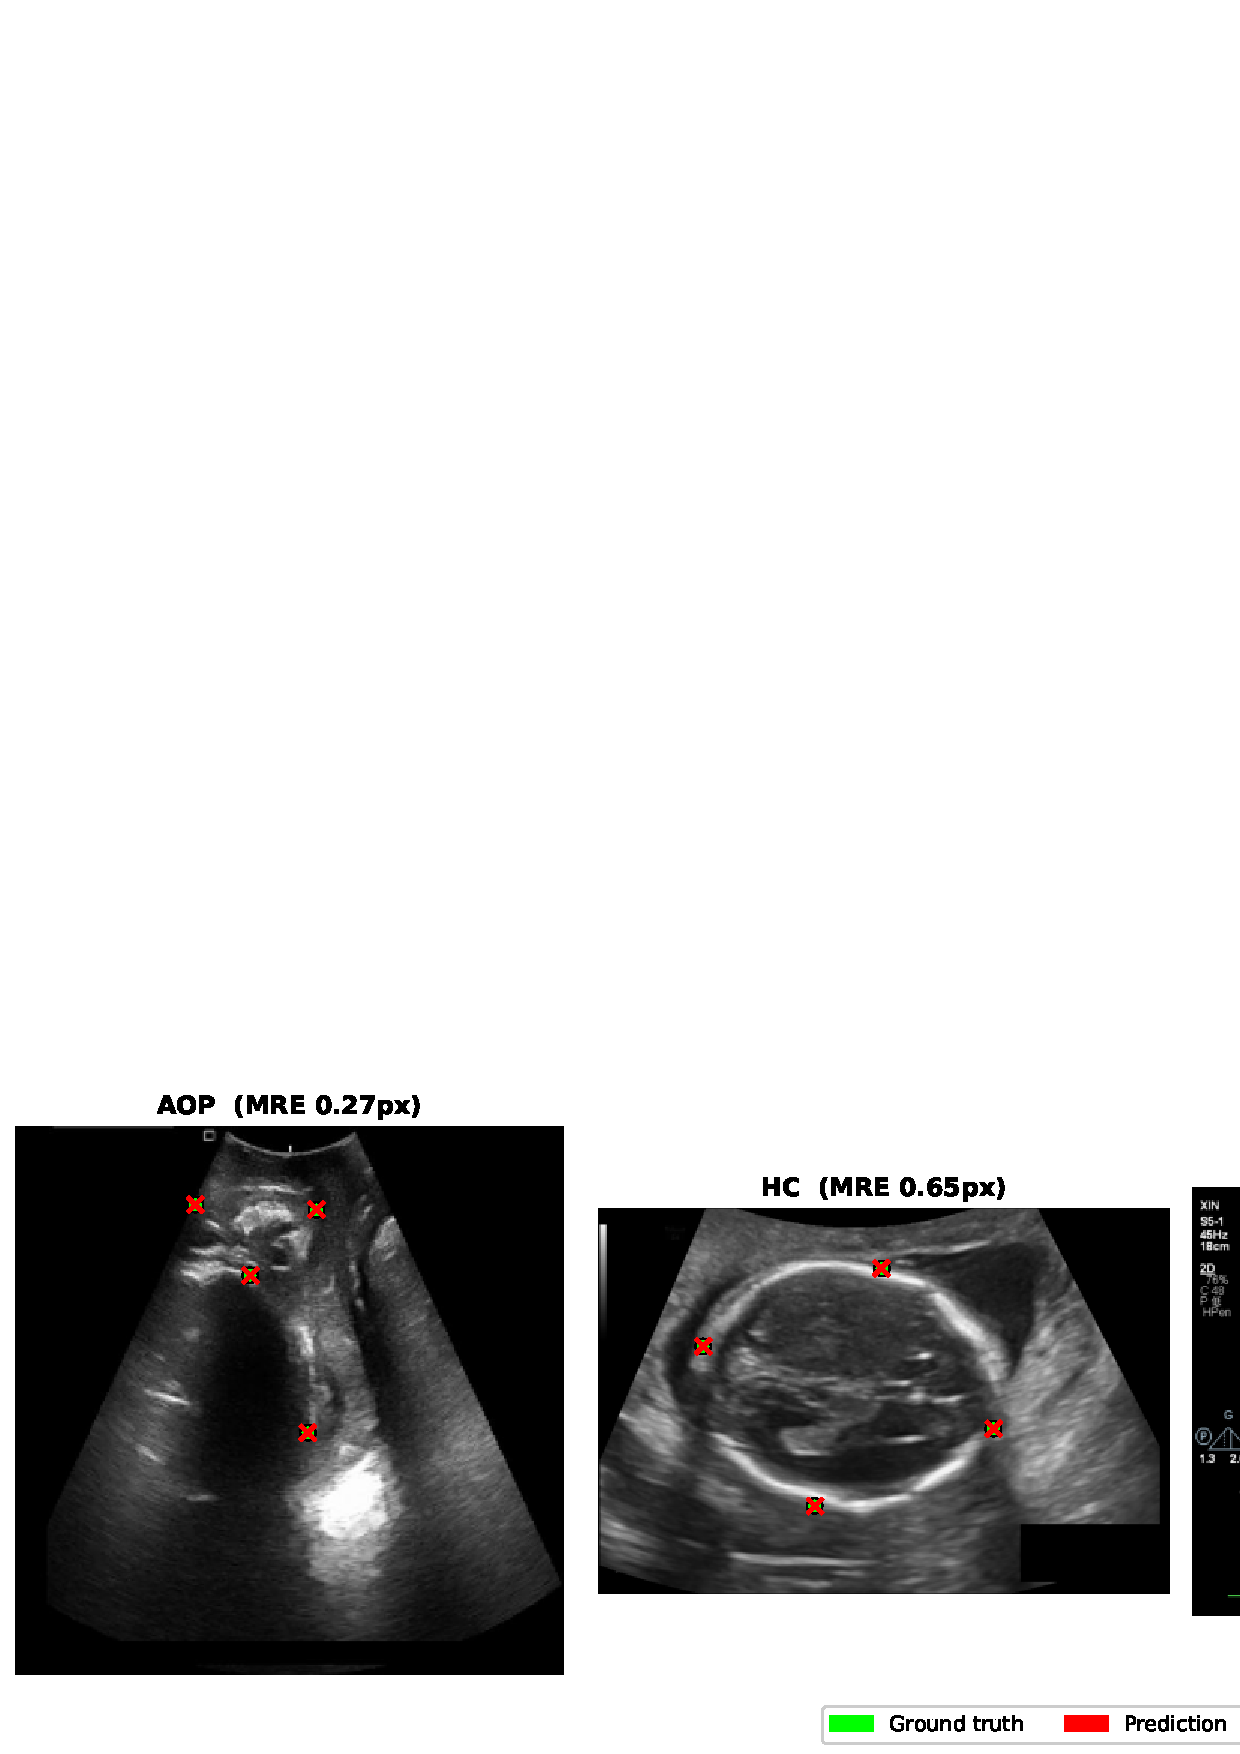
\includegraphics[width=\textwidth]{fig_best_per_task_row.pdf}
\caption{Representative high-performing validation examples for four tasks spanning different clinical domains. Ground-truth (green) vs.\ predicted (red) keypoints.}
\label{fig:best-per-task}
\end{figure}

\section{Conclusion}
We presented a two-stage DINOv2-HRNet pipeline for multi-task ultrasound landmark detection, coupling domain-targeted self-supervised adaptation with a top-down, multi-resolution HRNet-style neck to achieve competitive performance across nine heterogeneous clinical tasks. Future work includes a stratified 5-fold ensemble with multi-scale/intensity test-time augmentation, and ablating the neck's multi-level fusion, head design, and fine-tuning depth.

\begin{credits}
\subsubsection{\ackname} % Funding / acknowledgments, if any.
The A100 80GB GPU cloud instances (MedViLA) used to train and evaluate all models in this study were provided by the NVIDIA Academic Hardware Grant Program.
\subsubsection{\discintname}
The authors have no competing interests to declare that are relevant to
the content of this article.
\end{credits}

%
% ---- Bibliography ----
% BibTeX users: specify bibliography style 'splncs04' (Springer's LNCS
% style). Entries live in mybibliography.bib next to this file.
%
\clearpage
\bibliographystyle{splncs04}
\bibliography{mybibliography}

\end{document}
